\documentclass[10pt]{standalone}

\input{../tikzpic_packages.tex}
\usepackage{url}


\begin{document}
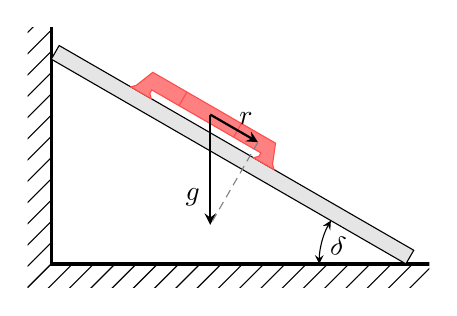
\begin{tikzpicture}[
scale=1, 
solid/.style={line width=.333mm, draw=red!40},
plate/.style={draw=black, fill=gray!20},
darrow/.style={stealth-stealth},
camera/.style={fill=black},
stativ/.style={very thick},
gecko/.style={draw=red!70, fill=red!50},
block/.style={draw, minimum width=3cm, minimum height=1cm, fill=gray!10},
arrow/.style={-triangle 45},
cable/.style={rounded corners=5mm, smooth, double}
]

\def\l{5.2} % length of plate
\def\t{.2} % thickness of plate
\def\buf{.2} % Extra Length of housing
\def\r{1.1} % Radius for angle notes
\def\ls{.5} % Schraffur Laenge

\path[clip](-.3,3)rectangle(4.8,-.3);

% Housing
\draw[very thick] (\l+\buf,0)--(0,0)--(0,\buf+\l);
\foreach \pos in {0,.05,...,1.05}{
	\path (0,0)--(\l+\buf,0)coordinate[pos=\pos](x);
	\path (0,0)--(0,\l+\buf)coordinate[pos=\pos](y);
	\draw (x)--++(225:\ls);
	\draw (y)--++(225:\ls);	
}

% Ebene
\def\del{30} % Ebenenwinkel
\foreach \del/\opa in {30/1}{
	\begin{scope}[opacity=\opa]
	\pgfmathsetmacro{\x}{cos(\del)*\l}
	\pgfmathsetmacro{\y}{sin(\del)*\l}
	\draw[plate] (\x,0)--(0,\y)--++(90-\del:\t)--++(-\del:\l)coordinate[midway](PlaneMid)--++(-90-\del:\t);
	\draw[darrow] (\x-\r,0)arc(180:180-\del:\r);
	\pgfmathsetmacro{\delh}{0.5*\del}
	\path (\x,0)++(180-\delh:\r)node[right,rotate=-\delh]{$\delta$};
	\end{scope}
}





% Gecko
%\def\del{30}
\def\rl{.7}	% length of r-vec
\begin{scope}[rotate=-\del]
\draw[gecko] (PlaneMid)++(0,0)++(-.3,.1)--++(-1,0)--++(0,-.05)--++(0.05,-.05)--++(-0.3,0)--++(.05,0.05)--++(.1,.25)--++(.5,0)--++(0,-.2)--++(0,.2)--++(.8,0)coordinate[midway](GeckoMid)--++(0,-.2)--++(0,.2)--++(.5,0)--++(.1,-.25)--++(.05,-.05)--++(-.3,0)--++(.05,.05)--++(0,0.05)--cycle;

\draw[-stealth, black,thick] (GeckoMid)++(0,-.1)coordinate(GeckoMid)--++(\rl,0)node[near end, above]{$\bm{r}$}coordinate(help);
\end{scope}

\pgfmathsetmacro{\gl}{\rl*(sin(\del)+tan(90-\del)*cos(\del))} % length of g-vec
\draw[-stealth, thick] (GeckoMid)--++(0,-\gl)node[near end, left]{$\bm{g}$}coordinate(gg);
\draw[densely dashed, gray] (help)--(gg);

\path (GeckoMid)node{\tiny \centerofmass};


\end{tikzpicture}
\end{document}